\section{Pretraining experiments and scaling}
\label{sec:scaling}

We evaluate \mname{WT-MLP-Lag} against unpreconditioned \mname{Muon}, tuned input-only \mname{MuonT}, and all-diagonal output preconditioning (\mname{OD-All}) across three pretraining regimes: multi-seed confirmation at 130M (20 tokens per non-embedding parameter, TPP), fourfold horizon scaling at 130M (80 TPP, 10.74B tokens), and width transfer to 520M (20 TPP, 10.74B tokens). Across all three regimes, \mname{WT-MLP-Lag} lowers final held-out loss relative to \mname{MuonT}, extending \mname{MuonT}'s held-out gain over \mname{Muon}—$(\mathcal L_{\rm MuonT}-\mathcal L_{\rm WT})/(\mathcal L_{\rm Muon}-\mathcal L_{\rm MuonT})$, with denominators $0.0119$, $0.0103$, and $0.0090$ nats—by 29--51\%.

\subsection{Experimental setup}
\label{sec:testbed}

We train 32-layer, pre-RMSNorm SwiGLU Transformers on a 25.4B-token mixture of DCLM, StarCoderData, and Proof-Pile-2 in the Marin PyTorch suite~\citep{mohamadi2026toner}, using the Llama-3.1 vocabulary of 128,256 tokens, sequence length 4,096, document-isolated causal attention, and NVIDIA A100-40GB GPUs. Within every seed, all optimizer arms share parameter initialization and minibatch data ordering. The labels 130M and 520M denote models with approximately 134M ($\dm=512,\dff=2{,}048$) and 537M ($\dm=1{,}024,\dff=4{,}096$) non-embedding parameters (\Cref{tab:regimes}).

\suppressfloats[t]
\begin{table}[tbp]\centering\small
\setlength{\tabcolsep}{5.8pt}
\caption{\textbf{Pretraining regimes.} Params counts non-embedding parameters; TPP is tokens per non-embedding parameter. Fresh-seed confirmation uses seeds 1--3 after learning-rate selection and execution-path checks on seed 0.}\label{tab:regimes}
\begin{tabularx}{\textwidth}{@{}>{\raggedright\arraybackslash}Xrrrrrc@{}}
\toprule
Regime & Params & $\dm$ / $\dff$ & Tokens (TPP) & Batch / Steps & GPUs & Seeds \\
\midrule
130M controls \& LR bracket & 134M & 512 / 2,048 & 2.68B (20) & 0.5M / 5,120 & 8$\times$A100 & 0 \\
130M confirmation & 134M & 512 / 2,048 & 2.68B (20) & 0.5M / 5,120 & 8$\times$A100 & 1, 2, 3 \\
130M longer training & 134M & 512 / 2,048 & 10.74B (80) & 0.5M / 20,480 & 8$\times$A100 & 0 \\
520M width transfer & 537M & 1,024 / 4,096 & 10.74B (20) & 1.0M / 10,240 & 32$\times$A100 & 0 \\
\bottomrule\end{tabularx}
\end{table}


We evaluate completed models on held-out training-mixture cross-entropy $\Lsel$, C4 cross-entropy $\Lc$, and the unweighted macro average across 16 out-of-distribution Paloma domains $\Lpal$. To check whether gains persist throughout late training rather than appearing only at schedule end, we also report paired means over the 11 second-half evaluation checkpoints (Late-11; correlated trajectory observations rather than independent seeds). Differences are reported in millinats ($1\text{ mnat}=10^{-3}\text{ nats}$, negative favoring the row method). Because short-schedule proxy sweeps select overly aggressive learning rates that degrade full-budget runs (\Cref{sec:falsification}), we sweep $\eta\in\{0.01131,0.016,0.02263,0.032\}$ at the full 2.68B-token budget on seed 0, where all four core methods share the same strict interior optimum $\eta^*=0.0160$.

\begin{table}[!htb]\centering\small
\setlength{\tabcolsep}{1.5pt}
\caption{\textbf{Confirmatory and scaling results across fresh seeds, longer horizon, and greater width.} Held-out reports final cross-entropy $\Lsel$ in nats; all $\Delta$ columns report differences from same-regime Muon in millinats (negative favors the row method). MuonT applies input preconditioning only, so the gap between the MuonT and Muon2-ExpDiag rows isolates the output-side contribution. Late-11 averages the 11 second-half checkpoints; Wins counts the 16 Paloma domains improved over Muon. All four methods share their verified seed-0 optimum within each regime ($\eta^*=0.01600$ at 130M and 520M 20 TPP, and $0.01600\times4^{-0.3}=0.01056$ at 130M 80 TPP). Complete absolute losses and $\eta=0.02263$ replicates appear in \Cref{tab:absolute_results,tab:seeds}.}\label{tab:main_scaling}
\begin{tabularx}{\textwidth}{@{}>{\raggedright\arraybackslash}Xrrrrrrr@{}}
\toprule
& & (nats) & \multicolumn{4}{c}{Differences from Muon (millinats, $\downarrow$)} & OOD \\
\cmidrule(lr){4-7}
Method & LR $\eta$ & Held-out & $\Delta$ Held-out & Late-11 $\Delta$ & $\Delta$ C4 & $\Delta$ Paloma & Wins \\
\midrule
\addlinespace[2pt]\multicolumn{8}{@{}l}{\textit{130M confirmation: 20 TPP, 2.68B tokens, fresh seeds 1--3 (matched $\eta^*=0.0160$, paired mean $\pm$ SD)}}\\
Muon & 0.01600 & 3.2035 & $+0.00$ & $+0.00$ & $+0.00$ & $+0.00$ & --- \\
MuonT & 0.01600 & 3.1916 & $-11.91\pm1.40$ & $-23.26\pm2.07$ & $-11.79\pm0.98$ & $-11.49\pm4.18$ & 16/16 \\
Muon2-Diag & 0.01600 & 3.1919 & $-11.62\pm1.09$ & $-22.91\pm1.63$ & $-12.63\pm1.22$ & $-12.79\pm1.92$ & 16/16 \\
\rowcolor{rowtint}[0pt][0pt]\textbf{Muon2-ExpDiag} & 0.01600 & \textbf{3.1881} & $\mathbf{-15.41\pm2.18}$ & $\mathbf{-26.78\pm2.30}$ & $\mathbf{-15.64\pm1.80}$ & $\mathbf{-15.91\pm1.68}$ & \textbf{16/16} \\
\addlinespace[5pt]\multicolumn{8}{@{}l}{\textit{130M longer training: 80 TPP, 10.74B tokens, seed 0 (matched rate)}}\\
Muon & 0.01056 & 3.0778 & $+0.00$ & $+0.00$ & $+0.00$ & $+0.00$ & --- \\
MuonT & 0.01056 & 3.0675 & $-10.28$ & $-22.28$ & $-10.26$ & $-11.12$ & 15/16 \\
Muon2-Diag & 0.01056 & 3.0656 & $-12.19$ & $-23.85$ & $-12.82$ & $-13.71$ & 16/16 \\
\rowcolor{rowtint}[0pt][0pt]\textbf{Muon2-ExpDiag} & 0.01056 & \textbf{3.0636} & $\mathbf{-14.23}$ & $\mathbf{-26.82}$ & $\mathbf{-14.07}$ & $\mathbf{-16.78}$ & \textbf{16/16} \\
\addlinespace[5pt]\multicolumn{8}{@{}l}{\textit{520M width transfer: 20 TPP, 10.74B tokens, $\dm=1{,}024$, seed 0 (matched $\eta^*=0.0160$)}}\\
Muon & 0.01600 & 2.8528 & $+0.00$ & $+0.00$ & $+0.00$ & $+0.00$ & --- \\
MuonT & 0.01600 & 2.8438 & $-9.02$ & $-20.00$ & $-7.33$ & $-3.56$ & 15/16 \\
Muon2-Diag & 0.01600 & 2.8433 & $-9.52$ & $-21.97$ & $-9.52$ & $-2.90$ & 12/16 \\
\rowcolor{rowtint}[0pt][0pt]\textbf{Muon2-ExpDiag} & 0.01600 & \textbf{2.8392} & $\mathbf{-13.57}$ & $\mathbf{-24.68}$ & $\mathbf{-11.62}$ & $\mathbf{-11.19}$ & \textbf{16/16} \\
\bottomrule\end{tabularx}
\end{table}


\subsection{Multi-seed confirmation at 130M}
\label{sec:phase2}

On fresh 130M seeds 1--3 at the shared full-budget optimum $\eta^*=0.0160$, \mname{WT-MLP-Lag} outperforms both \mname{Muon} and \mname{MuonT} on every seed across held-out mixture, C4, Paloma macro loss, and Late-11 checkpoints (\Cref{tab:main_scaling}, \Cref{fig:scaling_traj}(a)). Relative to same-seed \mname{MuonT}, \mname{WT-MLP-Lag} lowers final held-out loss by $0.0035\pm0.0017$ nats (mean $\pm$ sample standard deviation across seeds), whereas purely diagonal \mname{OD-All} leaves held-out mixture loss essentially unchanged ($+0.0003\pm0.0004$ nats). Replicating both output methods on the same three seeds at the hotter grid point $\eta=0.02263$ preserves this separation ($0.0034\pm0.0015$ versus $0.0005\pm0.0005$ nats; \Cref{tab:absolute_results,tab:seeds}). Retaining cross-channel output correlations at hidden width—rather than coordinate scaling or learning-rate selection—therefore accounts for the 130M improvement.

The gain also holds when doubling the global batch size to 1M tokens: the checked 130M run improves over \mname{MuonT} by $0.0036$ nats on held-out mixture and $0.0040$ nats on C4 (a single-seed batch-size check rather than an additional multi-seed replication).

\subsection{Longer training at four times the token budget}
\label{sec:phase3}

Training the 130M model for 10.74B tokens (80 TPP) tests whether input-only \mname{MuonT} closes the gap given four times as much data. Following Marin's standard $T^{-0.3}$ token-horizon rule at fixed batch size~\citep{mohamadi2026toner}, we scale the shared 20-TPP optimum to $\eta=0.016\times4^{-0.3}=0.01056$: \mname{WT-MLP-Lag} finishes $0.0040$ nats lower than \mname{MuonT} on held-out mixture and remains ahead at every second-half checkpoint (\Cref{tab:main_scaling}, \Cref{fig:scaling_traj}(b)), while its out-of-distribution Paloma macro gain reaches $0.0057$ nats across all 16 domains (\Cref{fig:paloma}(a)). Scaling instead from the adjacent $\sqrt2$-step grid point $\eta=0.02263=0.016\sqrt2$ ($\eta=0.01493$, $\sqrt2\times$ higher) incurs a mid-training penalty and finishes worse on Paloma (\Cref{fig:scaling_traj}(b), \Cref{tab:absolute_results}), confirming that output preconditioning still requires horizon-appropriate learning rates.

\begin{figure}[t]
 \centering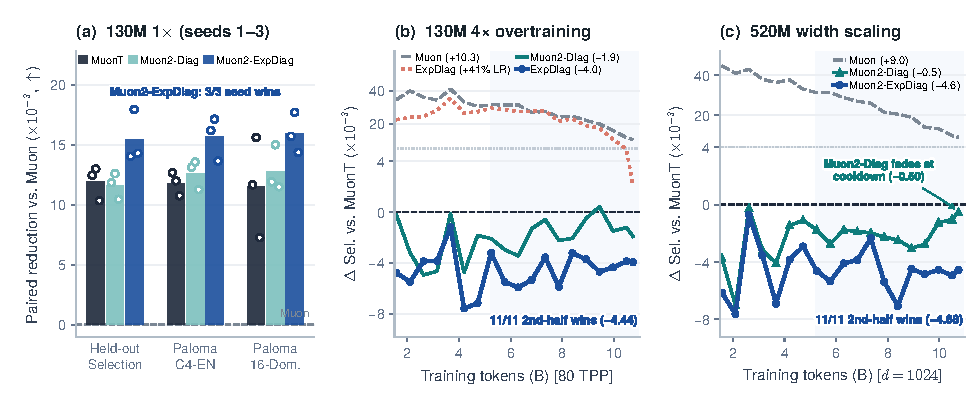
\includegraphics[width=\textwidth]{fig5_scaling_trajectories.pdf}
 \caption{\textbf{\mname{WT-MLP-Lag} improves over \mname{Muon} and \mname{MuonT} across fresh seeds, longer horizons, and greater width.}
 \textbf{(a)} Final loss reductions versus same-seed \mname{Muon} at 130M, 20 TPP; bars show three-seed means and open circles show individual seeds 1--3.
 \textbf{(b, c)} Held-out selection loss differences from \mname{MuonT} across 10.74B-token runs: 130M at 80 TPP and 520M at 20 TPP (one seed each; negative values favor the method). The hotter \mname{WT} curve in (b) illustrates horizon learning-rate sensitivity. Vertical axes compress the positive range above the dotted line.}
 \label{fig:scaling_traj}
\end{figure}

\subsection{Width transfer to 520M separates dense from all-diagonal outputs}
\label{sec:phase4}

Doubling model width to $\dm=1{,}024$ ($\dff=4{,}096$) cleanly separates width-thresholded dense outputs from purely diagonal outputs (\Cref{tab:main_scaling}, \Cref{fig:scaling_traj}(c)). Checking $\eta\in\{0.016,0.02263\}$ across all four methods at 520M selects the same shared optimum $\eta^*=0.016$ for every optimizer (\Cref{tab:absolute_results}). At this matched rate without output-side retuning, \mname{WT-MLP-Lag} lowers final held-out loss by $0.0046$ nats below \mname{MuonT} ($0.0043$ nats on C4) and leads at all 11 second-half checkpoints, whereas \mname{OD-All} gains only $0.0005$ nats on held-out mixture as its mid-training advantage fades during cooldown (at the hotter $\eta=0.02263$ rate, \mname{WT-MLP-Lag} still leads \mname{MuonT} by $0.0028$ nats while \mname{OD-All} finishes $0.0006$ nats worse; \Cref{tab:absolute_results}).

Per-domain evaluation on Paloma sharpens this contrast (\Cref{fig:paloma}(b), \Cref{tab:paloma_full}): at $\eta^*=0.016$, \mname{WT-MLP-Lag} improves over \mname{MuonT} in all 16 domains ($-7.63$ mnats macro mean), whereas \mname{OD-All} improves in 12 domains, regresses on four, and finishes worse than \mname{MuonT} overall ($+0.66$ mnats). Because Paloma domains share training and evaluation influences, win counts summarize out-of-distribution breadth within a run rather than independent replications, and two model widths do not establish an asymptotic scaling law.

\begin{figure}[t]
 \centering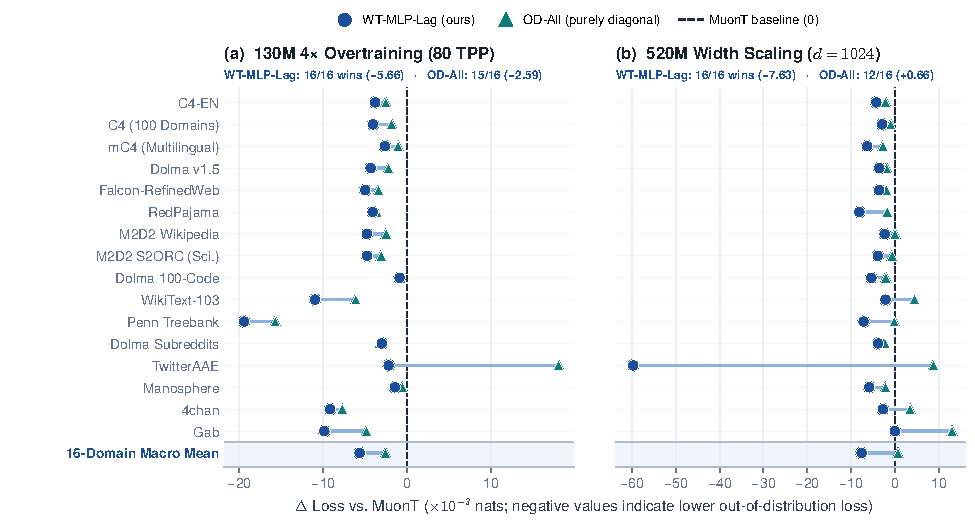
\includegraphics[width=\textwidth]{fig6_paloma_domains.pdf}
 \caption{\textbf{Retaining dense hidden-width output factors improves out-of-distribution loss across Paloma domains.}
 Final per-domain loss differences from \mname{MuonT} (negative values favor the method). \textbf{(a)} At 130M, 80 TPP, \mname{WT-MLP-Lag} wins 16/16 domains. \textbf{(b)} At 520M, 20 TPP, \mname{WT-MLP-Lag} wins 16/16 domains ($-7.63$ mnats macro) while \mname{OD-All} wins 12/16 ($+0.66$ mnats macro). Bottom rows show unweighted 16-domain macro means; horizontal scales differ across panels, and each regime uses one seed.}
 \label{fig:paloma}
\end{figure}
